\section{Results}

It is difficult to compare our results directly to literature, due to hardware limitations resulting in a maximum number of 
simulated neutrons that is far below what would be required for more natural geometries. Instead, we can make observations 
about the behaviour of the simulation output, and comment on whether it is aligned with what we would expect to occur.

\subsection{U-235 Simulations}

\subsubsection{Density Variation}

\begin{figure}[h!]
    \centering
    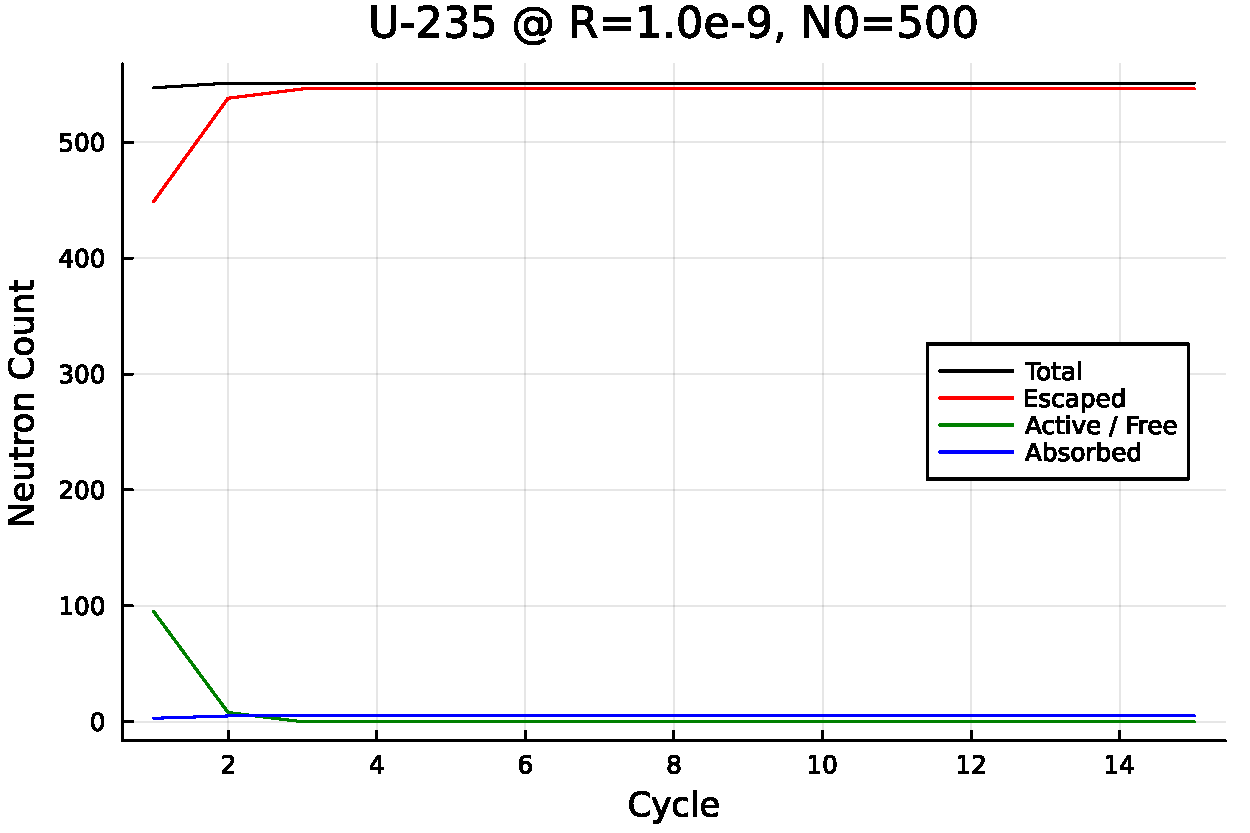
\includegraphics[scale=0.7]{imgs/neutron-count-uranium-large-sphere.pdf}
    \caption{A ``large'' sphere with radius $10^{-9}$cm, and a starting population of $500$ neutrons, run for 15 simulation 
    cycles.}
\end{figure}

\begin{figure}[h!]
    \centering
    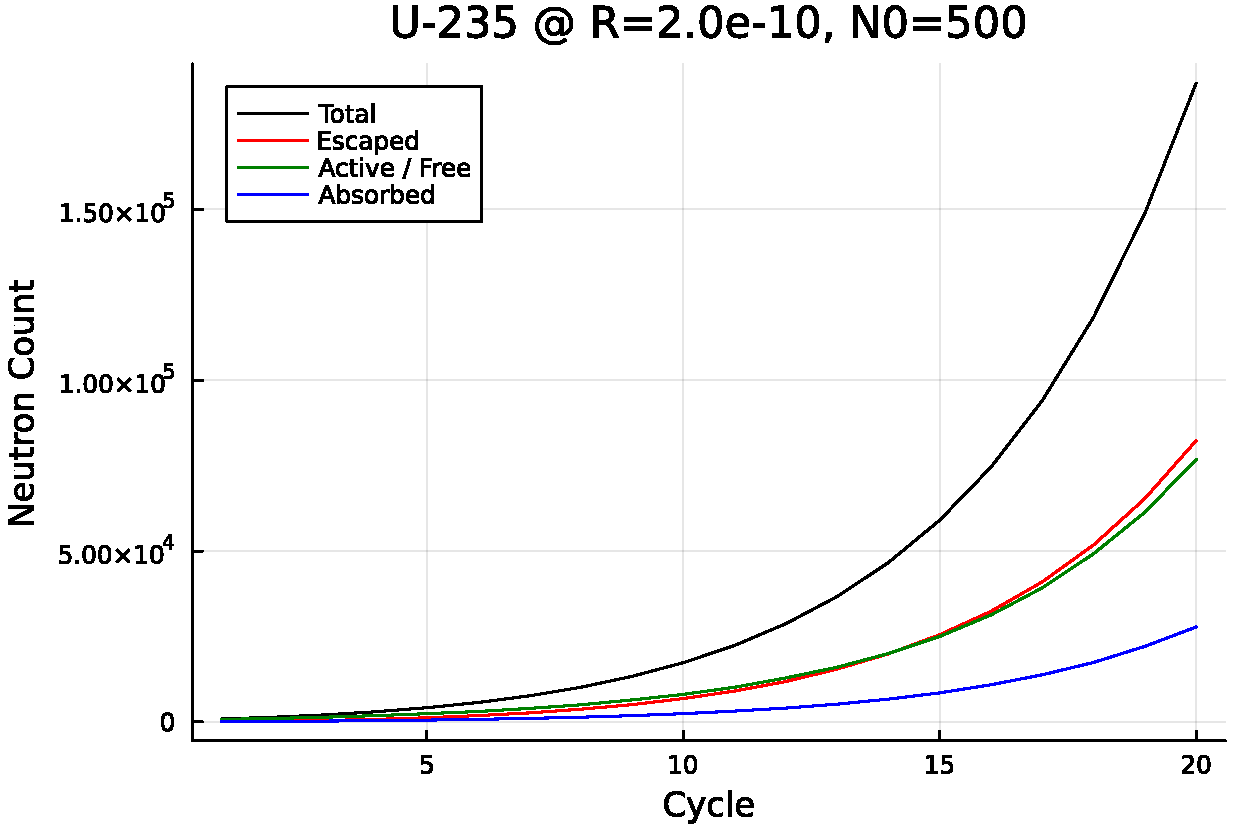
\includegraphics[scale=0.7]{imgs/neutron-count-uranium-medium-sphere-3-long.pdf}
    \caption{A ``medium'' sphere with radius $2 \cdot 10^{-10}$cm, and a starting population of $500$ neutrons, run for 20 simulation 
    cycles.}
\end{figure}

\begin{figure}[h!]
    \centering
    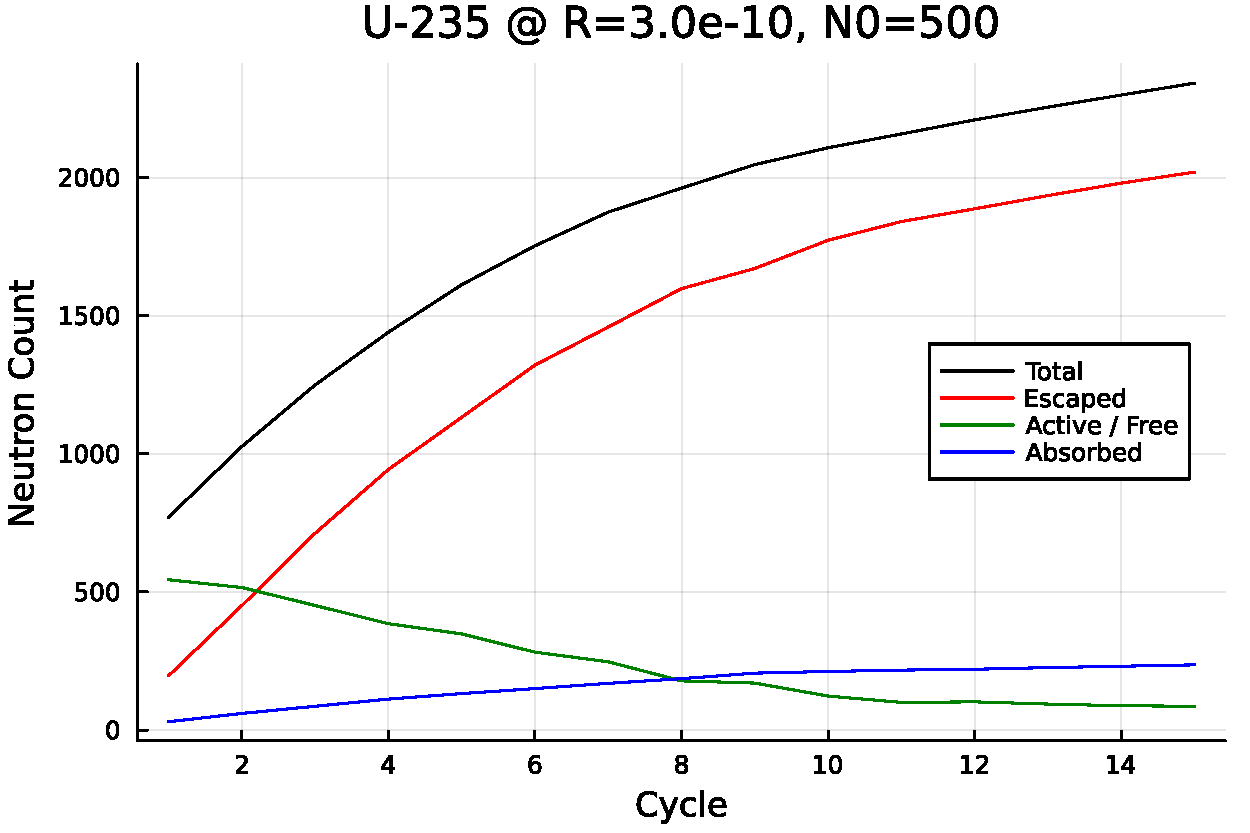
\includegraphics[scale=0.7]{imgs/neutron-count-uranium-medium-sphere-2.pdf}
    \caption{Another ``medium'' sphere with radius $3 \cdot 10^{-10}$cm, and a starting population of $500$ neutrons, run for 15 simulation 
    cycles.}
\end{figure}

\subsubsection{Critical Density Analysis}

Figures 4.1 - 4.3 show how different populations of neutrons in the medium grow under the dynamics of the system they're in. The only 
property that varies between these graphs is the radius of the sphere of Uranium in which the $500$ neutrons interact. Figure 
4.1 shows that almost all our neutrons escape almost immediately, while some are absorbed. No sustained fission reaction 
occurs in this case - we might posit that the sphere is too large (and thus the neutrons too sparse in our Uranium mass) to 
interact to a degree which encourages the production of other neutrons. This would be supported by the fact that the total population 
of neutrons remains largely unchanged from the initial count of $500$. 

This is in stark contrast to what we observe in, say, figure 4.2. Here we see sphere of smaller radius (increasing density),
and observe that our neutron population grows in what appears to be an exonential manner. Here, we are observing a self-sustaining 
fission reaction which has become super-critical. While some neutrons are still escaping, we see that the number of active neutrons 
is still growing exponentially, and so the reaction will self sustain. 

Figure 3.3 shows a more middle ground between the two. Theoretically it is possible to have a fission reaction system which is self sustaining,
without being super-critical or sub-critical. In practice, however, this is impossible as it requires a perfect balance of conditions which 
is not feasible in the real world. This figure depicts behaviour approaching that boundary, where the population of neutrons eventually decays 
to a sub-critical state, however does so at a slower rate than figure 4.1 which had a sphere of larger radius and so reached that state of 
non-reaction much faster.

We can see the relationship between radius of the sphere and the neutron population growth rate more clearly in figure \ref{uranium-total}. 

\begin{figure}[h!]
    \centering
    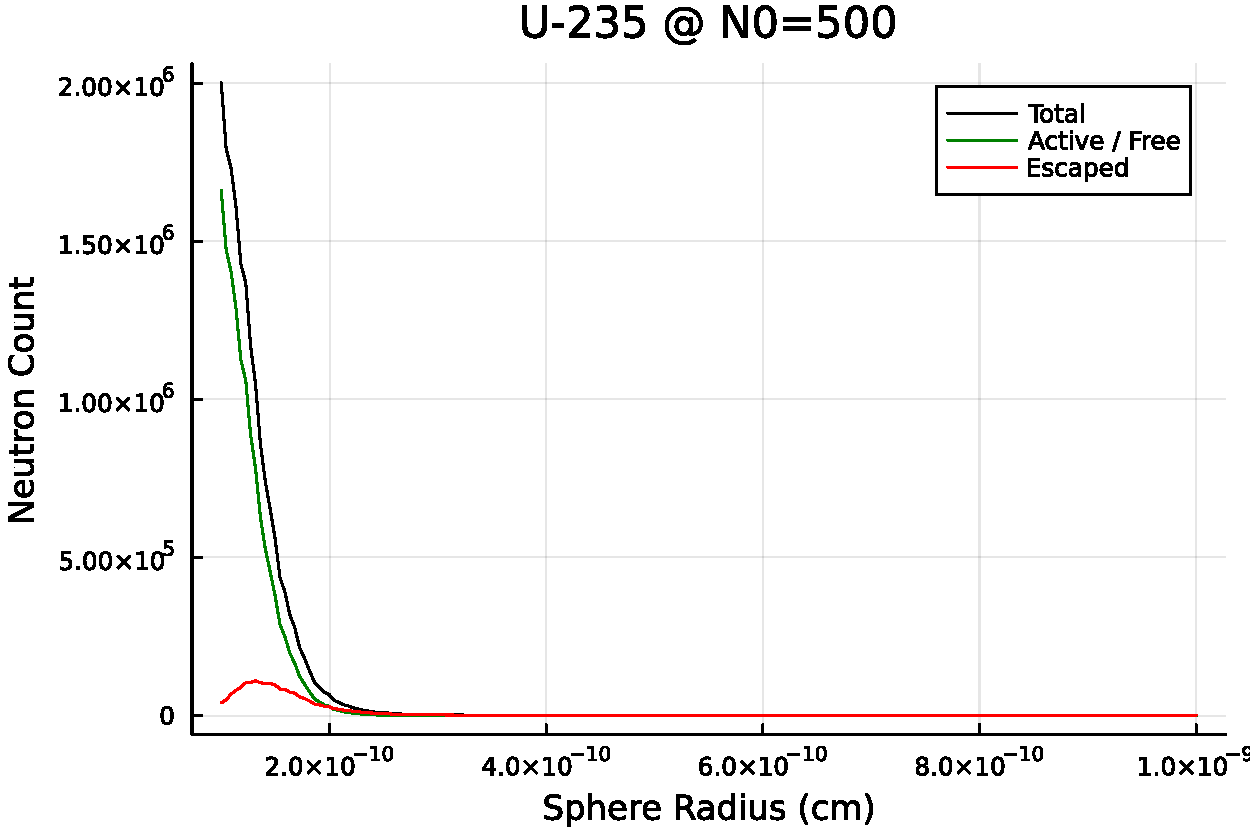
\includegraphics[scale=0.7]{imgs/radius-variation-uranium.pdf}
    \caption{Neutrons present in a mass of Uranium condensed into sphere of given radius (i.e. density is leftwards increasing in 
    the graph).}
    \label{uranium-total}
\end{figure}

We can clearly identify the trend we expect to see here. There is a point (around $3 \cdot 10^{-10} \text{cm}$) for which 
a sphere of greater radius will not result in a burn up situation - i.e., the number of neutrons either remains the same or 
decreases such that the reaction fizzles out. For spheres with a radius smaller than this, however, we see an exponential rise in the amount 
of neutrons as radius decreases. This is consistent with behaviour expected from super-critical systems, that is to say, 
it identifies the critical density for Uranium (when there are that many neutrons present). As we stated in our limitations, 
the number of neutrons present is incredibly unrealistic, and so we are unable to determine from this what the actual 
critical density of Uranium might be, unfortunately. However we are still able to identify behaviour, as the system scales nonetheless.

Note that there seems to be a dip in escaped neutrons as the sphere continues to decrease in radius. This is a misnomer, and 
is actually due to floating point errors - this comes about in the calculation of the euclidean distance of a neutron from 
the origin, and as distances decrease in size these values become smaller, until the code can no longer support their precision.

\subsection{Pu-239 Simulations}

\subsubsection{Density Variation}

\begin{figure}[h!]
    \centering
    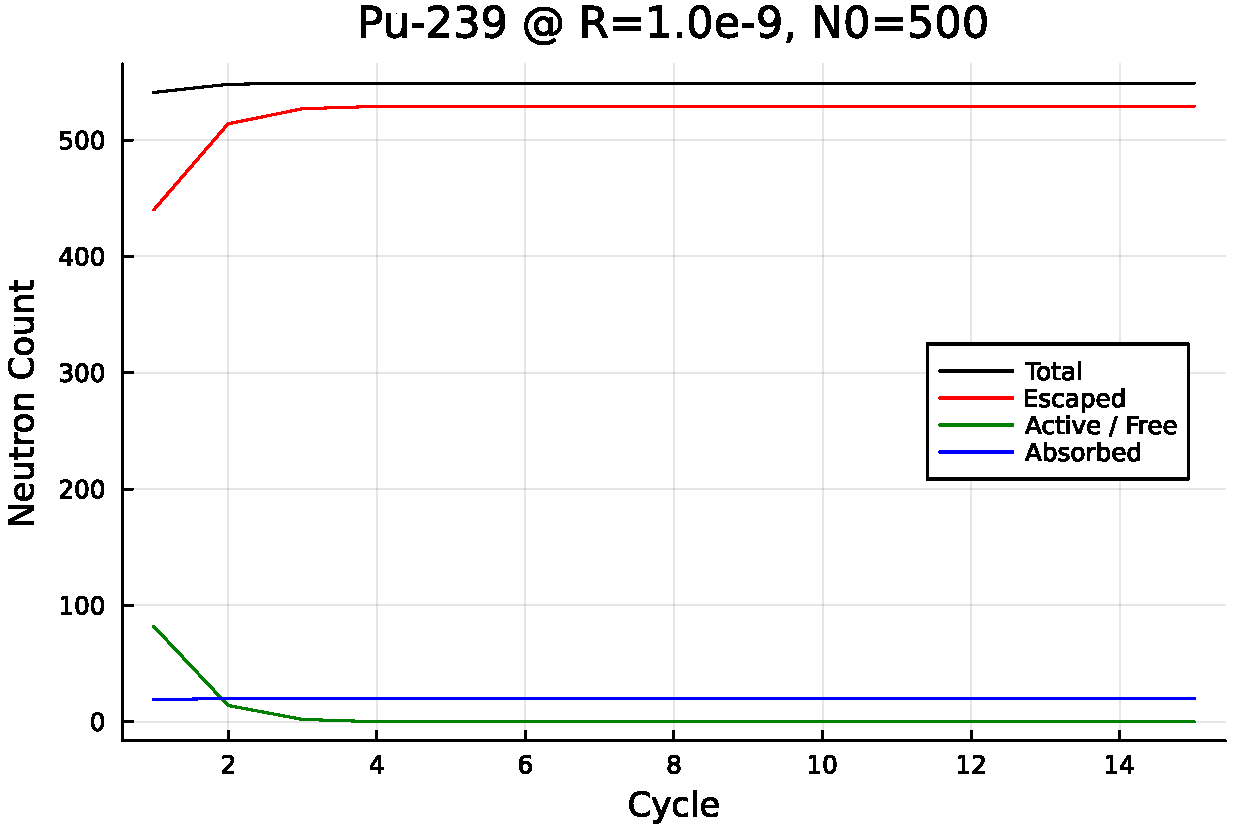
\includegraphics[scale=0.7]{imgs/neutron-count-plutonium-large-sphere.pdf}
    \caption{A ``large'' sphere with radius $10^{-9}$cm, and a starting population of $500$ neutrons, run for 15 simulation 
    cycles.}
\end{figure}

\begin{figure}[h!]
    \centering
    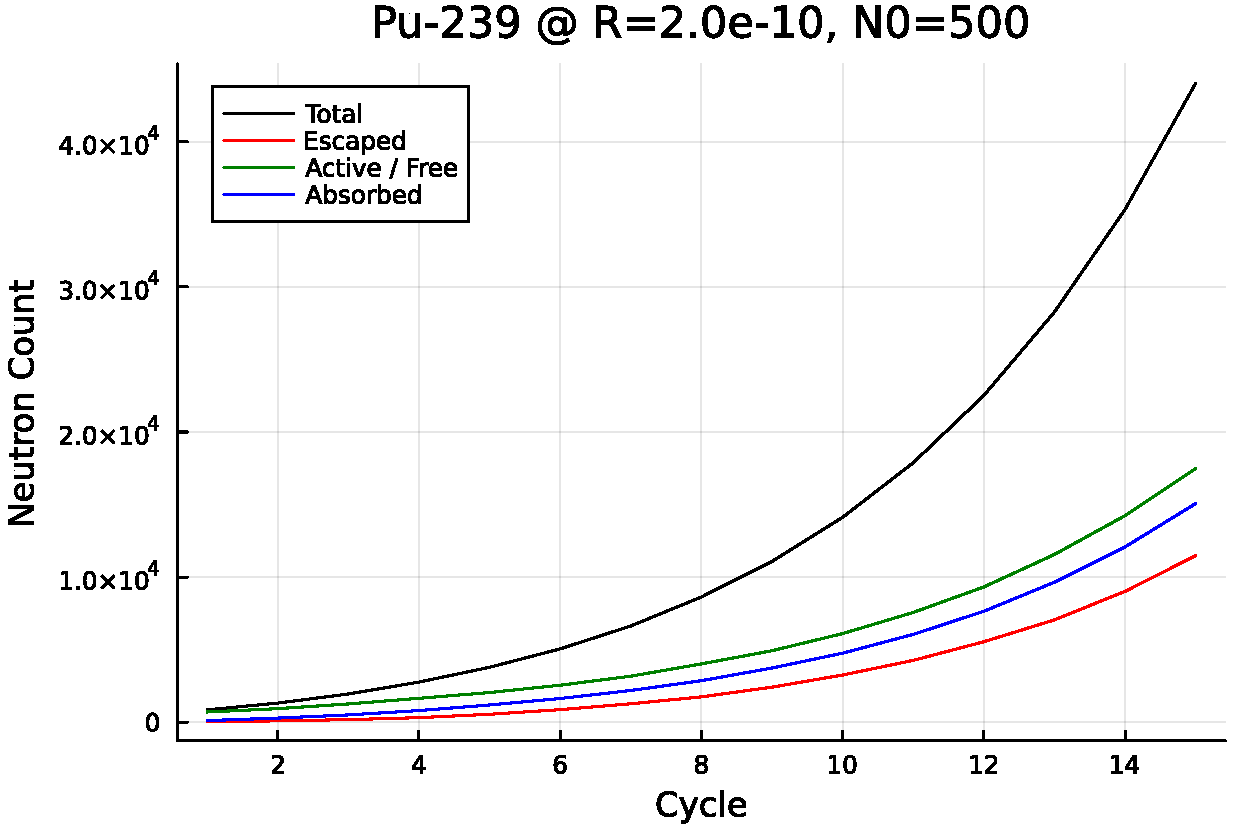
\includegraphics[scale=0.7]{imgs/neutron-count-plutonium-medium.pdf}
    \caption{A ``medium'' sphere with radius $2 \cdot 10^{-10}$cm, and a starting population of $500$ neutrons, run for 20 simulation 
    cycles.}
\end{figure}

\begin{figure}[h!]
    \centering
    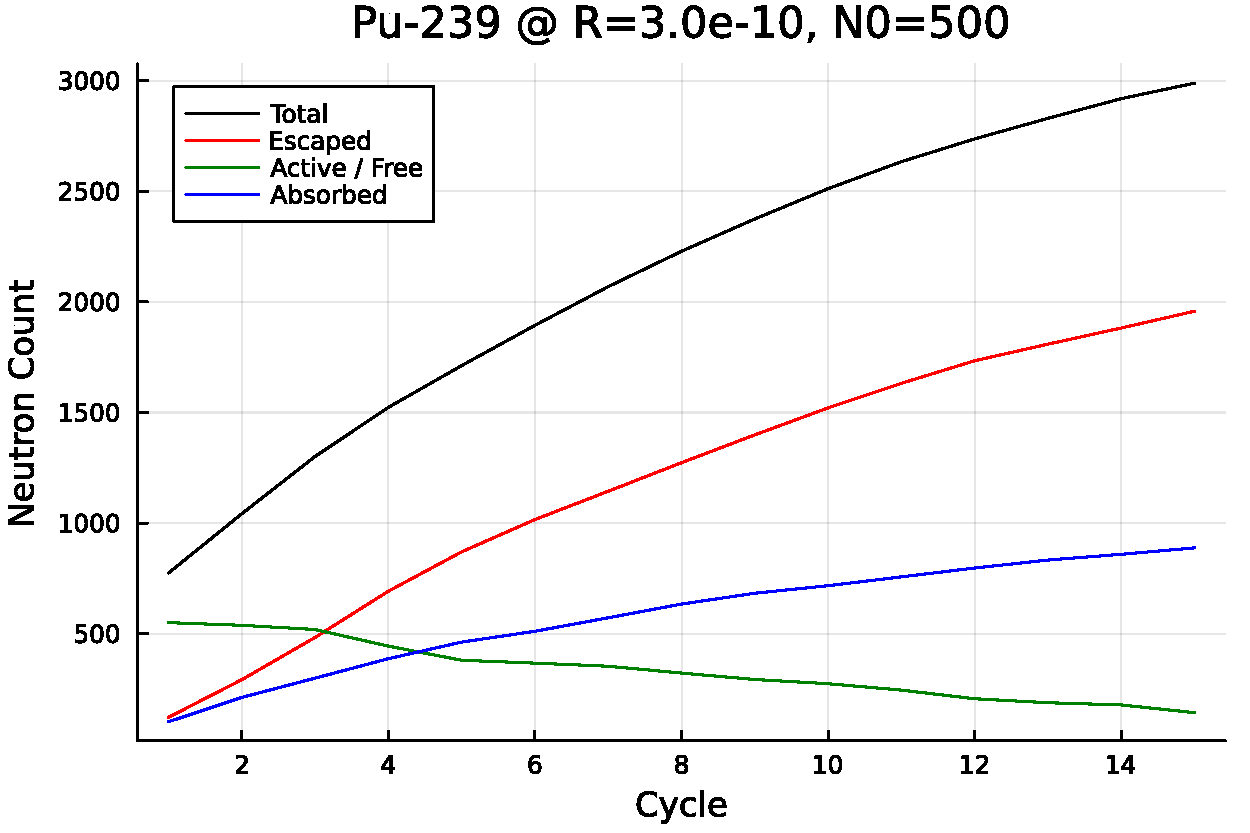
\includegraphics[scale=0.7]{imgs/neutron-count-plutonium-medium-2.pdf}
    \caption{Another ``medium'' sphere with radius $3 \cdot 10^{-10}$cm, and a starting population of $500$ neutrons, run for 15 simulation 
    cycles.}
\end{figure}

\subsubsection{Critical Density Analysis}

We largely include Plutonium in our simulations for two reasons: 1. because the bomb developed at Los Alamos had a Plutonium core, and 
it seemed only fitting to include a Plutonium simulation given the origins of the work in this; and 2. so we have something to compare the 
Uranium simulations to. 

\textcolor{red}{TODO: generate the radius graph but for Plutonium as well, then copy paste in here. Shouldn't need to change any text, just 
generate the graph}

When it comes to the Plutonium results, we see much the same behaviour as we did for Uranium, and for the same reasons. We only have 
to note that the orders to which the neutrons grow is somewhat greater for Uranium than for Plutonium. For example, for a sphere 
of radius $2 \cdot 10^{-10}\text{cm}$ Plutonium grew to a population of approximately 40000 neutrons, whereas Uranium sat 
comfortably at approximately 200000. If we recall back to our table which described the average cross section data for 
Uranium and Plutonium, we note that the average cross section values for capture and fission events are both greater for Plutonium 
than for Uranium. That is to say, a thermal neutron, on average, will have to travel farther through a Plutonium medium in order 
to experience a fission event, than it would if it were in a Uranium medium. Additionally, from these values, the probability 
of a fission reaction occurring sits at approximately $78$\% for Plutonium, whereas it sits at approximately $85$\% for Uranium.
Thus, we would expect there to be more fission reactions for a Uranium medium, and thus more opportunity for neutron development. The 
trend therefore is similarly consistent for comparisons between materials.